\providecommand{\main}{../..}
\documentclass[\main/notes.tex]{subfiles}

\begin{document}
	\setcounter{chapter}{8}
	\chapter{Knowledge Management and Specialised Information Systems}
	\chaptermark{Knowledge Management Systems}
		\section{Knowledge Management Systems}
			\begin{definition}{Knowledge}
				The awareness and understanding of a set of information, and the ways that information can be made useful, to support a specific task or reach a decision.
			\end{definition}
			\begin{definition}{Knowledge Management System (KMS)}
				An organised collection of people, procedures, software, databases and devices, used to create, store, share and use the organisation's knowledge and experience.
				\begin{indentparagraph}
					\begin{description}
						\item[Explicit Knowledge] Knowledge that is objective, and can be measured in reports, papers, and rules.
						\item[Tacit Knowledge] Knowledge that is hard to measure and document, and typically is not objective or formalised.
					\end{description}
					Many organisations actively attempt to convert tacit knowledge to explicit knowledge, to make the knowledge easier to measure, document, and share with others.
				\end{indentparagraph}
			\end{definition}
			\begin{sidenote}{Creating Knowledge}
				\begin{enumerate}
					\item When an individual learns directly from another individual, in an apprentice type relationship, tacit knowledge is created from tacit knowledge.
					\item When two pieces of explicit knowledge are combined.
					\item When an expert writes a book teaching others, explicit knowledge is being created from tacit knowledge.
					\item When someone reads that book, and (eventually) becomes an expert themselves, tacit knowledge has been created by explicit knowledge.
				\end{enumerate}
			\end{sidenote}
			\subsection{Obtaining, Storing, Sharing, and Using Knowledge}
				\begin{definition}{Chief Knowledge Officer}
					A top-level executive who helps the organisation use a KMS to create, store and use knowledge, to achieve organisational goals.
				\end{definition}
				After knowledge is created, it is often stored in a \concept{knowledge repository}.

				Using a KMS begins with locating the organisation's knowledge. This is often done using a \concept{knowledge map or directory} that points the knowledge worker to the needed knowledge.

		\section{Artificial Intelligence}
			\begin{definition}{Artificial Intelligence}
				Computers with the ability to mimic or duplicate the functions of the human brain.
			\end{definition}
			\begin{definition}{Artificial Intelligence Systems}
				People, procedures, hardware, software, data, and knowledge needed to develop computer systems and machines that demonstrate characteristics of intelligence.
			\end{definition}
			\subsection{The Nature of Intelligence}
				\begin{definition}{Intelligent Behaviour}
					The ability to:
					\begin{itemize}
						\item Learn from experience and apply the knowledge acquired from experience.
						\item Handle complex situations.
						\item Solve problems when important information is missing.
						\item Determine what is important.
						\item React quickly and correctly to a new situation.
						\item Understand visual images.
							\begin{indentparagraph}
								\begin{description}
									\item[Perceptive System] A system that approximates the way a person sees, hears, and feels objects.
								\end{description}
							\end{indentparagraph}
						\item Process and manipulate symbols
						\item Be creative and imaginative
						\item Use heuristics
					\end{itemize}
				\end{definition}
			\pagebreak
			\subsection{The Difference Between Natural and Artificial Intelligence}
				\begin{center}
					\begin{tblr}{colspec={ | >{\raggedright}X[3]|X[1]|X[1]|X[1]|X[1]| }, row{1}={font=\bfseries}, row{2}={font=\bfseries}, row{odd[2]}={table even}}
						\toprule
						\SetCell[r=2]{c} Ability to
							  & \SetCell[c=2]{c} Natural Intelligence
								    &     & \SetCell[c=2]{c} Artificial Intelligence & \\
							  & \SetCell[c=1]{c}Low & \SetCell[c=1]{c}High & \SetCell[c=1]{c}Low & \SetCell[c=1]{c}High\\
						\midrule
						Use sensors &  & \SetCell[c=1]{c}X & \SetCell[c=1]{c}X & \\
						Be creative and imaginative &  & \SetCell[c=1]{c}X & \SetCell[c=1]{c}X & \\
						Learn from experience &  & \SetCell[c=1]{c}X & \SetCell[c=1]{c}X & \\
						Adapt to new situations &  & \SetCell[c=1]{c}X & \SetCell[c=1]{c}X & \\
						Afford the cost of acquiring intelligence &  & \SetCell[c=1]{c}X & \SetCell[c=1]{c}X & \\
						Acquire a large amount of external information & & \SetCell[c=1]{c}X & & \SetCell[c=1]{c}X \\
						Use a variety of information sources & & \SetCell[c=1]{c}X & & \SetCell[c=1]{c}X \\
						Make complex calculations & \SetCell[c=1]{c}X & & & \SetCell[c=1]{c}X\\
						Transfer information & \SetCell[c=1]{c}X & & & \SetCell[c=1]{c}X\\
						Make a series of calculations rapidly and accurately & \SetCell[c=1]{c}X & & & \SetCell[c=1]{c}X \\
						\bottomrule
					\end{tblr}
				\end{center}
			\subsection{The Major Branches of Artificial Intelligence}
				\begin{definition}{Expert Systems}
						Hardware and software that stores knowledge, and makes inferences, similar to a human expert.
				\end{definition}
				\begin{definition}{Robotics}
					Mechanical or computer devices that perform tasks requiring a high degree of precision, or that are tedious or hazardous for humans.

					Robots are used to the `three Ds' -- dull, dirty, and dangerous jobs.
				\end{definition}
				\begin{definition}{Vision Systems}
					The hardware and software that permit computers to capture, store, and manipulate visual images.
				\end{definition}
				\begin{definition}{Natural Language Processing}
					Processing that allows the computer to understand and react to statements and commands made in a `natural' language, such as English.
					\begin{indentparagraph}
						\begin{description}
							\item[Voice recognition] Converting sound waves into words.
						\end{description}
					\end{indentparagraph}
				\end{definition}
				\begin{definition}{Learning Systems}
					A combination of software and hardware that allows the computer to change how it functions, or react to situations based on feedback it receives.
				\end{definition}
				\begin{definition}{Neural Networks}
					A computer system that attempts to simulate the function of a human brain.

					Uses massive parallel processors in an architecture that is based on the human brain's own mesh-like structure.
				\end{definition}
				\begin{definition}{Genetic Algorithm}
					Also called a \concept{genetic program}. An approach to solving large, complex problems, in which a number of related operations or models change and evolve until the best one emerges.
				\end{definition}
				\begin{definition}{Intelligent Agent}
					Also called an \concept{intelligent robot}, or \concept{bot}. Programs and a knowledge base used to perform a specific task for a person, a process, or another program.
				\end{definition}

		\section{Expert Systems}
			An expert system outputs a recommendation based on answers given to it by users (who are not experts in the field)
			\begin{sidenote}{When to Use Expert Systems}
				\begin{itemize}
					\item Provide a high potential payoff or significantly reduce downside risk.
					\item Capture and preserve irreplaceable human expertise.
					\item Solve a problem that is not easily solved using traditional programming techniques.
					\item Develop a system which is more consistent than human experts.
					\item Provide expertise needed at a number of locations at the same time, or in a hostile environment that is dangerous to human health.
					\item Provide expertise that is expensive or rare.
					\item Develop a solution faster than human experts can.
					\item Provide expertise needed for training and development to share the wisdom and experience of human experts with many people.
				\end{itemize}
			\end{sidenote}
			\subsection{Components of an Expert System}
				\begin{sidenote}{Components of an Expert System}
					An expert system consists of a collection of integrated and related components, including a knowledge base, an inference engine, an explanation facility, a knowledge base acquisition facility, and a user interface.
					\begin{center}
						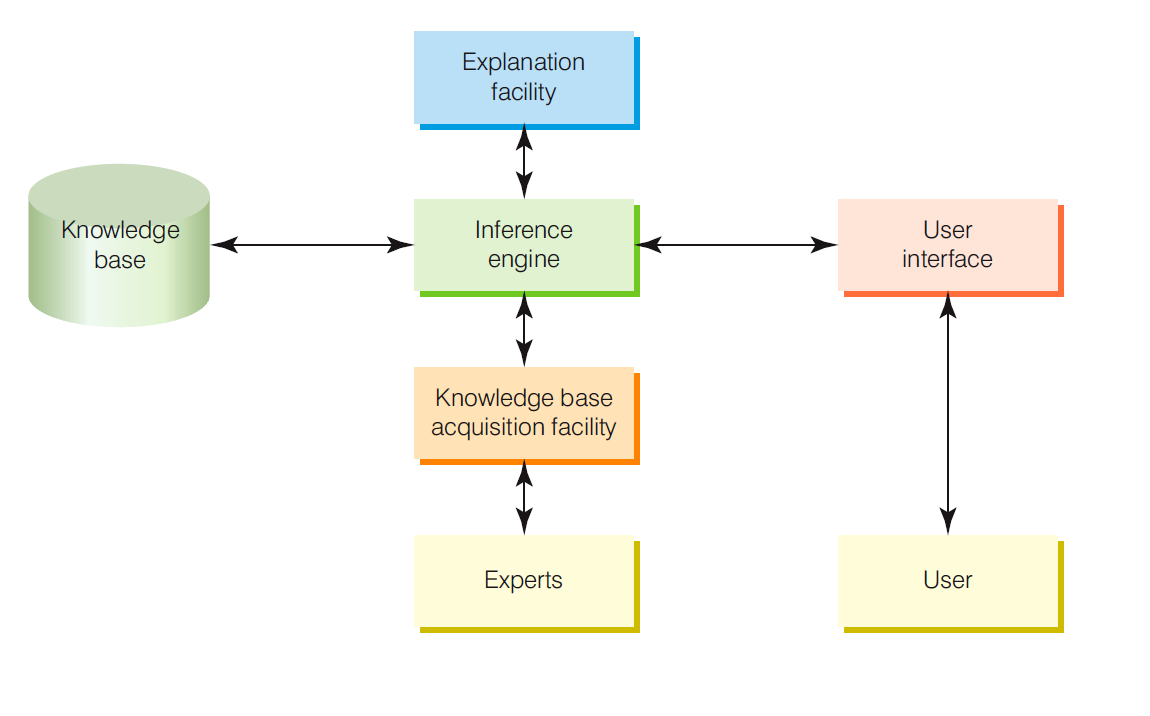
\includegraphics[width=0.7\textwidth]{chapter09/expert_systems.png}
					\end{center}
				\end{sidenote}
				\subsubsection{The Knowledge Base}
					\begin{definition}{Knowledge Base}
						A component of an expert system that stores all relevant information, data, rules, cases, and relationships used by the expert system.

						A natural extension of a database, and a decision support system.
					\end{definition}
					\begin{sidenote}{Tools and Techniques to Create a Knowledge Base}
						\begin{itemize}
							\item Assembling human experts
							\item Fuzzy logic -- allow knowledge and relationships that are not precise or exact.
							\item Rules: a conditional statement that links conditions to actions or outcomes.
								\begin{indentparagraph}
									\begin{description}
										\item[IF-THEN statements] Rules that suggest certain conclusions.
									\end{description}
								\end{indentparagraph}
							\item Cases
						\end{itemize}
					\end{sidenote}
				\subsubsection{The Inference Engine}
					\begin{definition}{Inference Engine}
						Part of the expert system that seeks information and relationships from the knowledge base, and provides answers, predictions, and suggestions the way a human expert would.
					\end{definition}
					\begin{definition}{Backward Chaining}
						The process of starting with conclusions and working backwards to the supporting facts.
					\end{definition}
					\begin{definition}{Forward Chaining}
						The process of starting with the facts and working forwards to the conclusions.
					\end{definition}
				\subsubsection{The Explanation Facility}
					\begin{definition}{Explanation Facility}
						Component of an expert system that allows a user of decision maker to understand how the expert system arrived at certain conclusions or results.
					\end{definition}
				\subsubsection{The Knowledge Acquisition Facility}
					\begin{definition}{Knowledge Acquisition Facility}
						Part of the expert system that provides convenient and efficient means of capturing and storing all the components of the knowledge base.
					\end{definition}
			\subsection{Expert Systems Development}
				\begin{definition}{Domain}
					The area of knowledge addressed by the expert system.
				\end{definition}
				\begin{definition}{Domain Expert}
					The individual or group who has the expertise of knowledge one is trying to capture in the expert system.

					They can usually do the following:
					\begin{multicols}{2}
						\begin{itemize}[nosep]
							\item Recognise the real problem
							\item Develop frameworks for problem-solving
							\item Formulate theories about the situation
							\item Learn from experience
							\item Develop and use general rules to solve a problem
							\item Solve problems quickly and efficiently
							\item Know when to break the rules or general principles
							\item Know what is and is not important in solving a problem
							\item Explain the situation and solutions of problems to others
						\end{itemize}
					\end{multicols}
				\end{definition}
				\begin{definition}{Knowledge Engineer}
					A person who has training or experience in the design, development, implementation, and maintenance of an expert system.
				\end{definition}
				\begin{definition}{Knowledge User}
					The person or group that uses and benefits from the expert system.
				\end{definition}
				\subsubsection{Expert Systems Development Tools and Techniques}
					\begin{definition}{Expert System Shell}
						A collection of software packages and tools used to design, develop, implement and maintain expert systems.
					\end{definition}
			\subsection{Applications of Expert Systems and Artificial Intelligence}
				\begin{sidenote}{Applications of Expert Systems and Artificial Intelligence}
					\begin{multicols}{2}
						\begin{itemize}[nosep]
							\item Credit granting and loan applications
							\item Stock picking
							\item Catching cheats and terrorists
							\item Budgeting
							\item Games
							\item Information management and retrieval
							\item AI and expert systems embedded in products
							\item Plant layout and manufacturing
							\item Hospitals and medical facilities
							\item Help desk and assistance
							\item Employee performance evaluation
							\item Virus detection
							\item Repair and maintenance
							\item Shipping
							\item Marketing
							\item Warehouse optimisation
							\item Diagnosis
						\end{itemize}
					\end{multicols}
				\end{sidenote}

		\section{Virtual Reality}
			\begin{definition}{Virtual Reality}
				Originally referred to immersive virtual reality, in which the user becomes fully immersed in an artificial, 3D world that is completely generated by a computer.

				A virtual realty system enables one or more users to move and react in a computer-simulated environment.
			\end{definition}
			\begin{definition}{Augmented Reality}
				The combination of computer generated data with stimuli from the real world.
			\end{definition}
			\subsection{Interface Devices}
				\begin{sidenote}{Devices in VR}
					To see in a virtual world, users wear a \concept{head-mounted display (HMD)}, with screens directed at each eye. The HMD also contains a \concept{position tracker} to monitor the location of the user's head, and the direction the user is looking.

					Users hear sounds in the virtual world through speakers mounted above to behind the screens. Spatial audio is possible, allowing for position tracking. When a sound source in virtual reality is not directly in front of or behind the user, the computer transmits sounds to arrive a little or later at one ear.

					The \concept{haptic interface}, which relays touch and other physical sensations, is the least developed, and the most challenging. Currently, gloves and a position tracker are used.
				\end{sidenote}
			\subsection{Forms of Virtual Reality}
				\begin{sidenote}{Forms of Virtual Reality}
					VR can refer to applications that are not fully immersive, such as mouse-controlled navigation through a 3D environment in a graphics monitor.
					\begin{description}
						\item[Motion trackers] Monitor the movements of dancers or athletes for subsequent studies in immersive virtual reality.
						\item[Telepresence systems] Immerse a viewer in a real world that is captured by video cameras at a distant location, and allow for the remote manipulation of real objects via robot arms and manipulators.
					\end{description}
				\end{sidenote}

		\section{Exercises}
			\begin{exercise}{Self-Assessment}
				\begin{enumerate}[nosep]
					\item AI systems demonstrate characteristics of \concept{intelligence}.
					\item Two branches of AI are \concept{Expert Systems} and \concept{Robotics}.
					\item Research into robots that are the size of a grain of salt is called \concept{micro-robotics}.
					\item Systems like a Google search on a smartphone that allows users to give voice input are examples of \concept{natural language processing}.
					\item The component of an expert system that stores relevant data and rules is the \concept{knowledge base}.
					\item An application for an expert system is \concept{credit granting and loan applications}.
					\item HMD stands for \concept{head mounted display}.
					\item A program that solves a problem by evolving new solutions repeatedly is a \concept{genetic algorithm}.
					\item A program that attempts to simulate a human brain is a \concept{neural network}.
					\item A system that attempts to approximate the way a human feels is a \concept{perceptive system}.
				\end{enumerate}
			\end{exercise}

	\vbox{\rulechapterend}
\end{document}